
%(BEGIN_QUESTION)
% Copyright 2008, Tony R. Kuphaldt, released under the Creative Commons Attribution License (v 1.0)
% This means you may do almost anything with this work of mine, so long as you give me proper credit

Determine the amount of time needed for the capacitor voltage ($V_C$) to fall to the specified levels after the switch is thrown to the ``discharge'' position, assuming it had first been charged to full battery voltage:

$$\includegraphics[width=15.5cm]{i03247x01.eps}$$

% No blank lines allowed between lines of an \halign structure!
% I use comments (%) instead, so that TeX doesn't choke.

$$\vbox{\offinterlineskip
\halign{\strut
\vrule \quad\hfil # \ \hfil & 
\vrule \quad\hfil # \ \hfil \vrule \cr
\noalign{\hrule}
%
% First row
$V_C$ & Time  \cr
%
\noalign{\hrule}
%
% Third row
8 volts &  \cr
%
\noalign{\hrule}
%
% Fourth row
6 volts &  \cr
%
\noalign{\hrule}
%
% Fifth row
4 volts &  \cr
%
\noalign{\hrule}
%
% Sixth row
2 volts &  \cr
%
\noalign{\hrule}
} % End of \halign 
}$$ % End of \vbox


\vfil 

\underbar{file i03247}
\eject
%(END_QUESTION)





%(BEGIN_ANSWER)

This is a graded question -- no answers or hints given!
 
%(END_ANSWER)





%(BEGIN_NOTES)

When discharging from an initial voltage of 12 volts, the voltage across the capacitor will be described by the following inverse exponential equation:

$$V_C = 12 e^{-{t \over RC}}$$

Manipulating this equation to solve for $t$:

$${V_C \over 12} = e^{-{t \over RC}}$$

$$\ln {V_C \over 12} = -{t \over RC}$$

$$-RC \ln {V_C \over 12} = t$$



% No blank lines allowed between lines of an \halign structure!
% I use comments (%) instead, so that TeX doesn't choke.

$$\vbox{\offinterlineskip
\halign{\strut
\vrule \quad\hfil # \ \hfil & 
\vrule \quad\hfil # \ \hfil \vrule \cr
\noalign{\hrule}
%
% First row
$V_C$ & Time  \cr
%
\noalign{\hrule}
%
% Third row
8 volts & 1.31 s \cr
%
\noalign{\hrule}
%
% Fourth row
6 volts & 2.24 s \cr
%
\noalign{\hrule}
%
% Fifth row
4 volts & 3.55 s \cr
%
\noalign{\hrule}
%
% Sixth row
2 volts & 5.79 s \cr
%
\noalign{\hrule}
} % End of \halign 
}$$ % End of \vbox

%INDEX% Electronics review: RC circuit time constant calculations

%(END_NOTES)


